\documentclass[conference]{IEEEtran}
\IEEEoverridecommandlockouts
\usepackage{cite}
\usepackage{amsmath,amssymb,amsfonts}
\usepackage{algorithmic}
\usepackage{graphicx}
\usepackage{textcomp}
\usepackage{xcolor}
\usepackage{booktabs}
\usepackage{algorithm}
\usepackage{microtype}
\usepackage{enumitem}
\setlist{nosep,leftmargin=*}
\setlength{\textfloatsep}{7pt plus 1pt minus 1pt}
\setlength{\intextsep}{5pt plus 1pt minus 1pt}
\setlength{\floatsep}{5pt plus 1pt minus 1pt}
\setlength{\abovecaptionskip}{3pt}
\setlength{\belowcaptionskip}{3pt}
\usepackage{tikz}
\usetikzlibrary{shapes.geometric,arrows.meta,positioning}
\def\BibTeX{{\rm B\kern-.05em{\sc i\kern-.025em b}\kern-.08em
    T\kern-.1667em\lower.7ex\hbox{E}\kern-.125emX}}
\begin{document}

\title{Low-Latency Concept Drift Detection and Online Adaptation for High-Throughput Streaming Classification}

\author{\IEEEauthorblockN{Yash Patidar}
\IEEEauthorblockA{\textit{School of Computer Engineering} \\
\textit{Manipal Institute of Technology,} \\
\textit{Manipal Academy of Higher Education}\\
Manipal, Karnataka \\
yash8.mitmpl2024@learner.manipal.edu}
\and
\IEEEauthorblockN{Pragun Kakkar}
\IEEEauthorblockA{\textit{School of Computer Engineering} \\
\textit{Manipal Institute of Technology,} \\
\textit{Manipal Academy of Higher Education}\\
Manipal, Karnataka \\
pragun.mitmpl2024@learner.manipal.edu}
\and
\IEEEauthorblockN{Shantanu Singh}
\IEEEauthorblockA{\textit{School of Computer Engineering} \\
\textit{Manipal Institute of Technology,} \\
\textit{Manipal Academy of Higher Education}\\
Manipal, Karnataka \\
shantanu.mitmpl2024@learner.manipal.edu}
}

\maketitle

\begin{abstract}
Continuous, high-velocity data streams generated by IoT sensor networks and real-time transaction pipelines frequently suffer from concept drift, where the underlying statistical distribution shifts over time and degrades predictive accuracy.
Existing drift detection frameworks often incur heavy computational overhead or rely on static thresholds that produce high false-alarm rates during gradual, non-stationary shifts.
In this work, we present a lightweight concept drift detection and online adaptation framework designed for high-throughput streaming classification.
The detector is built from first principles upon the Page-Hinkley cumulative-sum test, augmented with a bias-corrected Exponentially Weighted Moving Average (EWMA) adaptive baseline that runs in strictly constant $O(1)$ time and memory per sample without sliding window buffers.
We integrate this detector into an interleaved test-then-train prequential pipeline paired with two incremental classifiers: a Hoeffding Adaptive Tree (HAT) and a streaming Logistic Regression (LR) pipeline.
We evaluate the framework across both synthetic (SEA concept generator) and real-world (Electricity Market, Elec2) streaming benchmarks.
On the SEA stream, both models detect an abrupt shift and recover to above 0.95 rolling accuracy within 1{,}200 to 1{,}400 samples.
On the real-world Elec2 benchmark, the streaming LR pipeline achieves a final rolling accuracy of 91.2\% while executing in only 10.61~$\mu$s per sample---7.3 times faster than HAT's 77.32~$\mu$s at 79.4\% accuracy.
Our results demonstrate that pairing an extremely fast linear learner with adaptive drift detection and hard resets can deliver superior accuracy and throughput compared to more complex tree-based models on recurring real-world streams.
\end{abstract}

\begin{IEEEkeywords}
concept drift, online learning, data stream mining, EWMA, Page-Hinkley test, Hoeffding Adaptive Tree, prequential evaluation
\end{IEEEkeywords}

\section{Introduction and Motivation}
Modern data-driven systems, including IoT sensor clusters, high-frequency financial platforms, and network intrusion monitors, process continuous streams of non-stationary data.
In these operational environments, the underlying data-generating distribution changes over time due to external environmental variations, evolving user habits, or economic fluctuations.
This phenomenon is known as \emph{concept drift}~\cite{mulimani2024}.
When concept drift occurs, models trained on past data experience substantial degradation in predictive accuracy~\cite{parasteh2024}.
Addressing this requires online learning architectures capable of updating incrementally with each incoming instance.

However, deploying adaptive machine learning models on high-throughput streaming pipelines introduces strict resource constraints.
A streaming classifier must process incoming records in real time under bounded per-sample execution latency and finite memory footprint~\cite{wan2024}.
Recent research has increasingly applied deep learning and representation-based methods to drift detection~\cite{wan2024, chambers2023}.
While these techniques can identify complex distribution shifts, they introduce large architectural footprints, significant computational latencies, and buffering requirements that are ill-suited for microsecond-scale data ingestion~\cite{wan2024}.
Conversely, traditional lightweight statistical detectors often rely on fixed, static decision thresholds that trigger false alarms during natural, gradual variance shifts in stationary streams~\cite{rum2026}.
Furthermore, standard reactive detection paradigms often suffer an extended performance collapse before gathering enough historical error evidence to trigger model adaptation~\cite{cano2026}.

This paper addresses this challenge by evaluating an efficient middle ground: a lightweight, constant-time concept drift detection and online adaptation framework.
We implement a Page-Hinkley cumulative-sum test enhanced with an adaptive bias-corrected Exponentially Weighted Moving Average (EWMA) running mean.
The detector operates in $O(1)$ time and memory per sample, dynamically adjusting to slow baseline trends while remaining sensitive to genuine concept shifts.
We couple this detector with two distinct incremental classifiers---a Hoeffding Adaptive Tree and a streaming Logistic Regression pipeline---and evaluate their performance under the prequential protocol on synthetic and real-world benchmarks.

The primary contributions of this work are as follows:
\begin{itemize}
    \item We implement an $O(1)$ constant-time and constant-memory Page-Hinkley concept drift detector with a bias-corrected EWMA running baseline, tracking error streams without sliding window buffers.
    \item We integrate the detector into an online prequential evaluation pipeline with model-specific adaptation hooks, comparing passive branch pruning in HAT against hard parameter resets in a streaming Logistic Regression pipeline.
    \item We evaluate the end-to-end framework on both synthetic (SEA) and real-world (Elec2) streaming datasets, recording detailed per-sample accuracy, recovery latency, and nanosecond-level processing time.
    \item We analyze the accuracy--latency Pareto frontier, demonstrating that an ultra-fast linear learner ($10.61\,\mu$s per sample) with hard resets outperforms a tree-based learner in both throughput and accuracy on recurring market drift.
\end{itemize}

The remainder of this report is organized as follows.
Section~II surveys recent literature on concept drift detection.
Section~III identifies the research gap, Section~IV states the formal problem, and Section~V lists the project objectives.
Section~VI describes the datasets and preprocessing procedures.
Section~VII details the proposed methodology and system architecture.
Section~VIII outlines the implementation details.
Section~IX presents the experimental results and baseline comparison.
Section~X discusses the findings, strengths, limitations, and alignment with project objectives.
Section~XI concludes the paper with directions for future scope.

\section{Literature Survey and Comparative Analysis}
The literature on concept drift detection reflects an ongoing trade-off between computational overhead and detection sensitivity.
Early statistical tests provided lightweight solutions but lacked adaptability to gradual distribution shifts.
In recent years, unsupervised representation learning and deep neural networks have gained popularity.
For example, Wan et al.~\cite{wan2024} introduced Maximum Concept Discrepancy (MCD) via contrastive learning to identify drift in high-dimensional spaces without supervision.
Chambers et al.~\cite{chambers2023} proposed AdaDeepStream, utilizing intermediate CNN activations to detect drift with limited true labels.
While effective in complex domains, deep approaches incur computational costs that create severe latency bottlenecks in high-velocity streams.

To reduce supervisory overhead, Fellicious et al.~\cite{fellicious2024} developed SUDS, an unsupervised drift sampling technique that selects homogeneous samples for model retraining, reducing annotation requirements by up to 80\%.
Wu and Xiong~\cite{wu2023} explored online incremental parameter updates in Bayesian classifiers for non-stationary environments, achieving low computational cost but showing sensitivity to class imbalance.
Aguiar and Cano~\cite{aguiar2023} applied meta-learning over sliding-window meta-features to dynamically select the most suitable drift detector, though this requires extensive offline meta-training.
Mulimani et al.~\cite{mulimani2024} combined ensemble learning with adaptive sliding windows in an online LightGBM framework, which performs well on gradual drift but responds sluggishly to abrupt changes.

To mitigate computational bottlenecks, recent research has returned to statistical and probabilistic formulations.
Parasteh and Sadaoui~\cite{parasteh2024} developed PRDD, a probabilistic detector tracking classifier confidence shifts in $O(1)$ time, demonstrating that tracking prediction error streams can yield high sensitivity without buffering raw data.
Rum and Song~\cite{rum2026} demonstrated that dynamically recalibrating reconstruction error thresholds using an EWMA baseline substantially suppresses false alarms in stationary and gradual drift streams.
Finally, proactive adaptation mechanisms have emerged: Guerrero Cano et al.~\cite{cano2026} developed proactive Hoeffding Tree variants estimating boundary trajectories to adapt before performance collapses, while Zhao and Shen~\cite{zhao2025} proposed PROCEED to proactively adjust model parameters for online time-series forecasting.
Table~\ref{tab:lit_survey} provides a comparative summary of these recent approaches.

\begin{table*}[htbp]
\caption{Comparative Analysis of Recent Concept Drift Detection Methodologies}
\begin{center}
\footnotesize
\begin{tabular}{|c|p{0.22\textwidth}|p{0.25\textwidth}|p{0.18\textwidth}|p{0.18\textwidth}|}
\hline
\textbf{Year} & \textbf{Title \& Authors} & \textbf{Proposed Methodology} & \textbf{Strengths} & \textbf{Limitations} \\
\hline
2023 & \textit{Online Learning of Bayesian Classifiers...} \cite{wu2023} & Online incremental algorithm updating Bayesian parameters per sample \cite{wu2023}. & Computationally economical; handles nonstationary streams \cite{wu2023}. & Lacks mechanisms for multi-class imbalanced data \cite{wu2023}. \\
\hline
2023 & \textit{AdaDeepStream: Streaming Adaptation...} \cite{chambers2023} & Uses CNN activations with streaming machine learning models for drift detection \cite{chambers2023}. & Rapid adaptation with minimal true-labeled samples \cite{chambers2023}. & High architectural overhead; depends on explicit drift detection \cite{chambers2023}. \\
\hline
2023 & \textit{Enhancing Concept Drift Detection...} \cite{aguiar2023} & Exploits meta-features from sliding windows to dynamically recommend drift detectors \cite{aguiar2023}. & Highly robust to class imbalance without relying on fixed detectors \cite{aguiar2023}. & Requires offline training of meta-models on large datasets \cite{aguiar2023}. \\
\hline
2024 & \textit{Online Detection and Adaptation...} \cite{mulimani2024} & Online LightGBM combining ensemble learning and adaptive sliding windows \cite{mulimani2024}. & Adaptive to both real and virtual concept drifts \cite{mulimani2024}. & Struggles with sudden, abrupt drift scenarios \cite{mulimani2024}. \\
\hline
2024 & \textit{A Probabilistic Approach for...} \cite{parasteh2024} & PRDD algorithm tracking posterior probability shifts using adaptive confidence \cite{parasteh2024}. & Constant time complexity $O(1)$ per sample; highly efficient \cite{parasteh2024}. & Dependent on the base classifier's probability calibration \cite{parasteh2024}. \\
\hline
2024 & \textit{Online Drift Detection with...} \cite{wan2024} & Computes Maximum Concept Discrepancy (MCD) via contrastive learning \cite{wan2024}. & Unsupervised operation; effective on complex, high-dimensional data \cite{wan2024}. & Deep encoder optimization requires significant resources \cite{wan2024}. \\
\hline
2024 & \textit{SUDS: A Strategy for Unsupervised...} \cite{fellicious2024} & Unsupervised drift sampling to select homogeneous samples for retraining \cite{fellicious2024}. & Reduces annotated data requirement by up to 80\% \cite{fellicious2024}. & Underperforms on artificial datasets lacking noise \cite{fellicious2024}. \\
\hline
2025 & \textit{PROCEED: Proactive Model Adaptation...} \cite{zhao2025} & Maps latent concept drift to parameter adjustments proactively to overcome feedback delays \cite{zhao2025}. & Anticipates drift before performance collapses \cite{zhao2025}. & Relies on historical drift patterns; struggles with out-of-distribution shifts \cite{zhao2025}. \\
\hline
2026 & \textit{An EWMA-Based Adaptive...} \cite{rum2026} & Dynamically updates reconstruction error thresholds using EWMA over autoencoders \cite{rum2026}. & Eliminates false alarms in stationary and gradual drift streams \cite{rum2026}. & Sensitive to tuning of the EWMA smoothing coefficient \cite{rum2026}. \\
\hline
2026 & \textit{Anticipating to Change...} \cite{cano2026} & Proactive Hoeffding Tree variants anticipating drift via boundary trajectory estimation \cite{cano2026}. & Prevents degradation proactively by maximizing class separability \cite{cano2026}. & Relies on linear boundary adjustments; struggles with erratic drifts \cite{cano2026}. \\
\hline
\end{tabular}
\label{tab:lit_survey}
\end{center}
\end{table*}

\section{Research Gap}
Existing research reveals two prominent gaps in streaming concept drift adaptation:
\begin{enumerate}
    \item \textbf{High computational cost versus rigid thresholding:} Deep learning and representation-based methods~\cite{wan2024, chambers2023} isolate complex drifts effectively but introduce heavy computational latency and memory buffering that make them impractical for high-velocity streaming. Conversely, lightweight statistical detectors often rely on static validation thresholds that fail to adjust to long-term gradual drift, resulting in frequent false alarms~\cite{rum2026}.
    \item \textbf{Reactive latency in online adaptation:} Most lightweight stream algorithms operate reactively, requiring a marked decline in predictive accuracy before accumulating sufficient statistical evidence to trigger an alarm~\cite{cano2026}. There is a lack of compact, constant-time adaptation frameworks that dynamically scale their internal baselines to detect drifts with minimal delay while maintaining strict microsecond-level processing throughput.
\end{enumerate}

\section{Problem Statement}
To design, implement, and evaluate a low-latency, resource-bounded concept drift detection and online adaptation framework for high-throughput data streams.
The proposed system must identify non-stationary distribution shifts in streaming classification models and initiate online model adaptation in real time, minimizing post-drift accuracy degradation while operating under strict $O(1)$ per-sample memory and time complexity constraints.

\section{Project Objectives}
The specific objectives of this project are:
\begin{itemize}
    \item \textbf{Objective 1:} Implement a constant-time $O(1)$ sequential concept drift detector based on the Page-Hinkley cumulative-sum test, tracking classification error streams without sliding window buffers~\cite{parasteh2024}.
    \item \textbf{Objective 2:} Integrate an adaptive thresholding baseline using a bias-corrected Exponentially Weighted Moving Average (EWMA) to continuously recalibrate the expected error level and suppress false alarms triggered by statistical noise~\cite{rum2026}.
    \item \textbf{Objective 3:} Couple the drift detector with incremental base learners (Hoeffding Adaptive Tree and streaming Logistic Regression) to execute online adaptation protocols upon receiving drift alarms~\cite{cano2026}.
    \item \textbf{Objective 4:} Evaluate the end-to-end framework under prequential protocol on synthetic and real-world streaming benchmarks, quantifying recovery latency, steady-state accuracy, and per-sample processing time~\cite{parasteh2024, rum2026}.
\end{itemize}

\section{Dataset Description and Preprocessing}
The framework is evaluated on two standard streaming benchmarks representing both controlled synthetic shifts and real-world recurring market drift.

\subsection{Synthetic SEA Concept Generator}
The SEA benchmark is a widely adopted synthetic streaming generator introduced by Street and Kim, implemented via the \texttt{river.datasets.synth.SEA} module.
Each instance consists of three independent continuous numerical attributes, $f_1, f_2, f_3 \in [0, 10]$.
The true concept boundary is governed by the linear inequality $f_1 + f_2 \le \theta$, where $\theta$ is a threshold parameter defining the binary target label $y \in \{0, 1\}$.
The third attribute $f_3$ is non-informative noise.
The class distribution is approximately balanced (50\% per class).

In our experimental pipeline, we simulate an abrupt concept shift by mixing two SEA concepts (\texttt{variant=0} with $\theta=8$, and \texttt{variant=1} with $\theta=9$) using a sigmoid-weighted mixing stream.
The transition is placed at sample index 25{,}000 with a narrow transition width ($w = 1$), producing an instantaneous concept change.
The total stream length is fixed at exactly 50{,}000 instances with a random generator seed of 42.
The instances are streamed in strictly sequential order without shuffling, preserving the temporal evolution of the stream.
Because the attributes are synthetic, uniformly distributed, and complete, no missing value imputation or offline scaling is applied.

\subsection{Electricity Market Benchmark (Elec2)}
The Elec2 benchmark is a real-world dataset collected from the Australian New South Wales (NSW) electricity market, originally compiled by Harries (1999) and provided by \texttt{river.datasets.Elec2}.
The dataset contains 45{,}312 instances collected at 30-minute intervals over a two-year period from May 1996 to December 1998.
Each instance comprises eight numerical attributes: date, day of week (1--7), time period (1--48), NSW electricity price, NSW electricity demand, Victoria (VIC) electricity price, VIC electricity demand, and scheduled electricity transfer between NSW and VIC.
The target variable is a binary classification label indicating whether the market price moved \textsc{down} (57.1\%) or \textsc{up} (42.9\%) relative to a 24-hour moving average.

The Elec2 stream contains naturally occurring concept drift caused by shifting consumer demand, regulatory changes, weather fluctuations, and transmission dynamics.
The instances are processed in strict chronological order to reflect real-time market operation.
No row-level filtering or instance reordering is performed.

\subsection{Preprocessing and Feature Engineering}
Data preprocessing is conducted in a streaming manner to respect online operational constraints:
\begin{itemize}
    \item \textbf{Streaming Standardization:} For the Logistic Regression learner, input features pass through \texttt{river.preprocessing.StandardScaler}, which maintains running accumulators of the mean and variance for each feature. As each sample $x_t$ arrives, the scaler transforms the raw feature values to zero mean and unit variance online before passing them to the linear model.
    \item \textbf{Scale Invariance in HAT:} For the Hoeffding Adaptive Tree, no feature normalization or scaling is applied. Decision trees evaluate split decisions using Hoeffding bounds on individual attribute coordinate rankings, which are invariant to monotonic feature scaling.
    \item \textbf{Target Encoding:} Binary string target labels (\textsc{down}/\textsc{up} in Elec2) are mapped to boolean/binary indicators $\{0, 1\}$.
    \item \textbf{Feature Engineering Statement:} No manual feature engineering (such as interaction terms, lag features, or polynomial expansions) was performed. Restricting the inputs to the original raw features ensures that measured differences in recovery and accuracy stem entirely from the learners' online adaptation mechanisms rather than handcrafted feature representations.
\end{itemize}

\section{Proposed Methodology and System Architecture}

\subsection{System Architecture and Pipeline Workflow}
The overall architecture operates on an interleaved test-then-train (prequential) loop, illustrated in Fig.~\ref{fig:architecture}.
The pipeline processes streaming data through five distinct stages:
\begin{enumerate}
    \item \textbf{Instance Ingestion:} An unlabelled sample $x_t$ arrives from the stream at time $t$.
    \item \textbf{Prequential Prediction:} The current model $f$ outputs a class prediction $\hat{y}_t = f(x_t)$, and its prediction is logged for rolling accuracy tracking.
    \item \textbf{Error Calculation:} The true label $y_t$ is observed, and a binary error signal is computed: $e_t = \mathbf{1}[\hat{y}_t \neq y_t] \in \{0, 1\}$.
    \item \textbf{Adaptive Drift Monitoring:} The error value $e_t$ is passed to the Page-Hinkley detector, which updates its EWMA running mean and cumulative-sum test statistic in $O(1)$ operations.
    \item \textbf{Adaptation and Model Update:} If the test statistic exceeds the detection threshold $\lambda$, a drift alarm is triggered: the model-specific adaptation callback $\textsc{Adapt}(f)$ is invoked, and the detector state is reinitialized. Finally, the model learns the sample via $f.\textsc{Learn}(x_t, y_t)$.
\end{enumerate}

\begin{figure}[htbp]
\centering
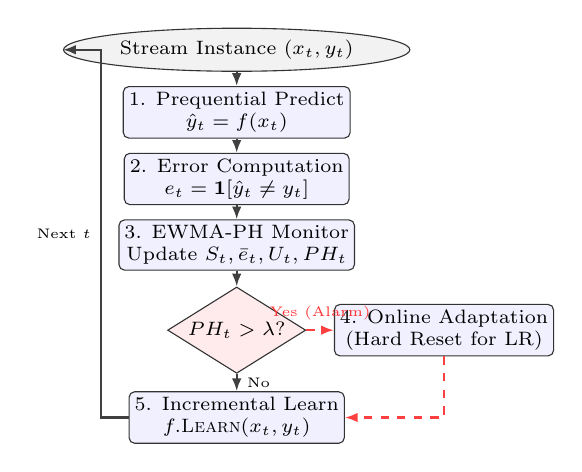
\begin{tikzpicture}[
    auto,
    node distance=0.22cm and 0.30cm,
    block/.style={rectangle, draw=black!80, fill=blue!6, rounded corners=2pt, font=\scriptsize, align=center, inner sep=2pt, minimum width=2.2cm, minimum height=0.40cm},
    decision/.style={diamond, draw=black!80, fill=red!8, font=\scriptsize, align=center, inner sep=1pt, aspect=1.6},
    io/.style={ellipse, draw=black!80, fill=gray!10, font=\scriptsize, align=center, inner sep=2pt},
    arr/.style={-{Latex[scale=0.7]}, thick, draw=black!75},
    redarr/.style={-{Latex[scale=0.7]}, thick, draw=red!75, dashed}
]
\node[io] (stream) {Stream Instance $(x_t, y_t)$};
\node[block, below=0.18cm of stream] (predict) {1. Prequential Predict\\$\hat{y}_t = f(x_t)$};
\node[block, below=0.18cm of predict] (error) {2. Error Computation\\$e_t = \mathbf{1}[\hat{y}_t \neq y_t]$};
\node[block, below=0.18cm of error] (ewma) {3. EWMA-PH Monitor\\Update $S_t, \bar{e}_t, U_t, PH_t$};
\node[decision, below=0.20cm of ewma] (check) {$PH_t > \lambda$?};
\node[block, right=0.35cm of check] (adapt) {4. Online Adaptation\\(Hard Reset for LR)};
\node[block, below=0.22cm of check] (learn) {5. Incremental Learn\\$f.\textsc{Learn}(x_t, y_t)$};

\draw[arr] (stream) -- (predict);
\draw[arr] (predict) -- (error);
\draw[arr] (error) -- (ewma);
\draw[arr] (ewma) -- (check);
\draw[redarr] (check) -- node[above, font=\tiny, text=red!80] {Yes (Alarm)} (adapt);
\draw[redarr] (adapt) |- (learn);
\draw[arr] (check) -- node[right, font=\tiny] {No} (learn);
\draw[arr] (learn.west) -- ++(-0.35,0) |- node[near start, left, font=\tiny] {Next $t$} (stream.west);

\end{tikzpicture}
\caption{System architecture and online prequential adaptation workflow.}
\label{fig:architecture}
\end{figure}

\subsection{Adaptive Drift Detection via EWMA-PH}
\label{sec:detector}
The concept drift monitor is formulated as a Page-Hinkley cumulative-sum change-point test with an exponentially weighted running baseline, implemented from first principles.
The detector operates on the scalar error signal $e_t \in \{0, 1\}$ through three recurrence relations:

\smallskip
\noindent\textbf{1. Bias-Corrected EWMA Baseline:}
A fading accumulator $S_t$ tracks the historical error rate:
\begin{equation}
S_t = \alpha \, S_{t-1} + (1 - \alpha) \, e_t, \quad S_0 = 0
\label{eq:ema_accum}
\end{equation}
where $\alpha \in (0, 1]$ is the fading smoothing factor.
To eliminate the severe startup underestimation typical of raw exponential smoothing when $t$ is small, we apply bias correction:
\begin{equation}
\bar{e}_t = \frac{S_t}{1 - \alpha^t}
\label{eq:ema_mean}
\end{equation}
When $t \ll 1 / (1 - \alpha)$, $\bar{e}_t$ acts like the cumulative arithmetic mean of observations; as $t$ grows, $\alpha^t \to 0$ and $\bar{e}_t$ smoothly relaxes into an exponential moving average with an effective memory horizon of $1 / (1 - \alpha)$ samples.
This formulation allows the detector to track gradual baseline drifts without chasing isolated outliers~\cite{rum2026}.

\smallskip
\noindent\textbf{2. Cumulative-Sum Statistic:}
The cumulative sum $U_t$ tracks the deviation of observed errors from the adaptive baseline, adjusted by a dead-band tolerance $\delta$:
\begin{equation}
U_t = U_{t-1} + \bigl(e_t - \bar{e}_t - \delta\bigr), \quad U_0 = 0
\label{eq:cusum}
\end{equation}
The parameter $\delta > 0$ introduces a negative drift under stationary conditions: $\mathbb{E}[e_t - \bar{e}_t - \delta] \approx -\delta < 0$.
Consequently, during stationary stream phases, $U_t$ drifts downward, preventing noise from accumulating into false alarms.

\smallskip
\noindent\textbf{3. Test Statistic and Drift Decision:}
The detector records the running historical minimum of $U_t$:
\begin{equation}
m_t = \min(m_{t-1}, U_t), \quad m_0 = 0
\label{eq:min}
\end{equation}
The Page-Hinkley test statistic $PH_t$ measures the rise of $U_t$ above its minimum:
\begin{equation}
PH_t = U_t - m_t
\label{eq:ph_stat}
\end{equation}
When a genuine concept drift occurs, $e_t$ increases abruptly while $\bar{e}_t$ lags behind.
The term $(e_t - \bar{e}_t - \delta)$ becomes persistently positive, causing $U_t$ to rise sharply away from its frozen historical minimum $m_t$.
A concept drift alarm is signaled the instant:
\begin{equation}
PH_t > \lambda
\label{eq:threshold}
\end{equation}
where $\lambda$ is the decision threshold.
Once triggered, the detector state $(S_t, \alpha^t, U_t, m_t)$ is reset to zero so that post-drift monitoring begins from a clean baseline.
All operations execute in $O(1)$ time and require storing only 6 floating-point state variables.

\subsection{Model Selection Justification}
We evaluate two contrasting incremental classifiers:
\begin{itemize}
    \item \textbf{Hoeffding Adaptive Tree (HAT):} A tree-based incremental learner from \texttt{river.tree}. HAT uses Hoeffding bounds to select split features and embeds internal ADWIN drift monitors at every branch. When an alternate subtree demonstrates superior accuracy over an existing branch, the branch is replaced. HAT provides high representational capacity for non-linear decision boundaries and has built-in passive adaptation.
    \item \textbf{Streaming Logistic Regression (LR):} A linear classifier from \texttt{river.linear\_model} trained via stochastic gradient descent (SGD), preceded by a streaming \texttt{StandardScaler}. LR represents an ultra-low-latency, constant-time learner with $O(d)$ complexity per sample.
\end{itemize}

The pairing of HAT and LR allows us to evaluate the trade-off between representational complexity and throughput.
Furthermore, choosing an EWMA-corrected Page-Hinkley detector over standard fixed-threshold Page-Hinkley or sliding-window methods is grounded in recent findings: static Page-Hinkley tests use a simple cumulative mean that becomes sluggish as $t$ grows, making them unable to detect later drifts~\cite{parasteh2024}.
Sliding-window approaches require maintaining buffers of historical records~\cite{mulimani2024}, whereas our EWMA formulation provides dynamic baseline recalibration in strict $O(1)$ space and time~\cite{rum2026, cano2026}.

\subsection{Online Adaptation Protocol}
Upon receiving a drift alarm ($PH_t > \lambda$), model-specific adaptation is triggered:
\begin{itemize}
    \item \textbf{Logistic Regression Pipeline:} SGD-based linear models possess no inherent forgetting mechanism; historical gradient updates remain embedded in the model weights. Therefore, we execute a \emph{hard parameter reset}, replacing both the \texttt{StandardScaler} and \texttt{LogisticRegression} instances with freshly initialized models.
    \item \textbf{Hoeffding Adaptive Tree:} No global model wipe is performed. HAT relies on its internal ADWIN-based alternate subtree pruning to replace underperforming subtrees gradually without discarding the entire tree hierarchy.
\end{itemize}

\subsection{Evaluation Metrics Formulation}
The following metrics are tracked across the streams:
\begin{itemize}
    \item \textbf{Rolling Accuracy ($\text{Acc}_t$):} Fraction of correct predictions over sliding window $W = 500$: $\text{Acc}_t = \frac{1}{\min(t, W)} \sum_{i = \max(1, t - W + 1)}^{t} \mathbf{1}[\hat{y}_i = y_i]$.
    \item \textbf{Final Steady-State Accuracy ($\text{Acc}_{\text{final}}$):} The rolling accuracy at stream conclusion ($t = N$).
    \item \textbf{Recovery Latency ($L_{\text{rec}}$):} Samples required after true drift $t^*$ to restore accuracy to $\ge 0.95$: $L_{\text{rec}} = \min \{ \Delta \ge 0 : \text{Acc}_{t^* + \Delta} \ge 0.95 \}$.
    \item \textbf{Detection Delay ($D$):} Distance between injected drift index $t^*$ and detector alarm $t_{\text{alarm}}$: $D = t_{\text{alarm}} - t^*$.
    \item \textbf{Mean Per-Sample Latency ($T_{\text{sample}}$):} Average wall-clock processing time per predict-learn cycle in microseconds ($\mu$s): $T_{\text{sample}} = \frac{1}{N} \sum_{t=1}^N \Delta t_{\text{sample}, t}$, recorded via \texttt{time.perf\_counter\_ns}.
    \item \textbf{Macro F1-Score:} Cumulative macro-averaged harmonic mean of precision and recall.
    \item \textbf{Drift Alarm Count ($K$):} Total number of drift alerts signaled across the stream.
\end{itemize}

Algorithm~\ref{alg:framework} outlines the complete prequential evaluation and adaptation routine.

\begin{algorithm}[htbp]
\caption{EWMA-PH Prequential Evaluation and Online Adaptation}
\label{alg:framework}
\footnotesize
\begin{algorithmic}[1]
\renewcommand{\algorithmicrequire}{\textbf{Input:}}
\REQUIRE Data stream $\mathcal{S}$, model $f$, detector parameters $(\alpha, \delta, \lambda)$, adaptation function $\textsc{Adapt}$
\STATE Initialize model $f$
\STATE Initialize detector state: $n \leftarrow 0, S_0 \leftarrow 0, U_0 \leftarrow 0, m_0 \leftarrow 0$
\FOR{each instance $(x_t, y_t) \in \mathcal{S}$}
    \STATE $t_{\text{start}} \leftarrow \textsc{CurrentTimeNano}()$
    \STATE $\hat{y}_t \leftarrow f.\textsc{Predict}(x_t)$
    \STATE $e_t \leftarrow \mathbf{1}[\hat{y}_t \neq y_t]$
    \STATE Update EWMA accumulator: $S_t \leftarrow \alpha S_{t-1} + (1 - \alpha) e_t$
    \STATE Compute baseline: $\bar{e}_t \leftarrow S_t / (1 - \alpha^t)$
    \STATE Update cumulative sum: $U_t \leftarrow U_{t-1} + (e_t - \bar{e}_t - \delta)$
    \STATE Update minimum: $m_t \leftarrow \min(m_{t-1}, U_t)$
    \STATE $PH_t \leftarrow U_t - m_t$
    \IF{$PH_t > \lambda$}
        \STATE $\textsc{Adapt}(f)$ \COMMENT{Reset LR or allow HAT pruning}
        \STATE Reset detector: $S_t \leftarrow 0, U_t \leftarrow 0, m_t \leftarrow 0$
    \ENDIF
    \STATE $f.\textsc{Learn}(x_t, y_t)$
    \STATE $\Delta t_t \leftarrow \textsc{CurrentTimeNano}() - t_{\text{start}}$
    \STATE Update rolling metrics $(\text{Acc}_t, \text{F1}_t, T_{\text{sample}})$
\ENDFOR
\end{algorithmic}
\end{algorithm}

\section{Implementation Details}
To facilitate reproducibility and clarity, this section outlines the software dependencies, codebase organization, hardware execution environment, and experimental parameter configurations.

\subsection{Software and Library Versions}
The framework was developed and executed using the following software stack:
\begin{itemize}
    \item \textbf{Programming Language:} Python 3.12 / 3.14 runtime environment.
    \item \textbf{Online Machine Learning:} \texttt{river} (v0.21.0), providing streaming estimators, metrics, and dataset loaders.
    \item \textbf{Scientific Computing:} \texttt{numpy} (v2.4.1) and \texttt{pandas} (v2.3.3) for telemetry handling.
    \item \textbf{Plotting:} \texttt{matplotlib} (v3.10.8) using the \texttt{seaborn-v0\_8-paper} style sheet.
\end{itemize}
The Page-Hinkley detector is implemented completely from first principles in \texttt{page\_hinkley.py} with zero dependencies on \texttt{river.drift}.

\subsection{Script Architecture in the Repository}
The implementation in \texttt{Project\_FML-main} is organized into modular scripts:
\begin{itemize}
    \item \texttt{page\_hinkley.py}: Implements the $O(1)$ Page-Hinkley detector with bias-corrected EWMA baseline via \eqref{eq:ema_accum}--\eqref{eq:ph_stat}, tracking 6 scalar variables ($n, S_t, \alpha^t, \bar{e}_t, U_t, m_t$).
    \item \texttt{stream\_evaluation.py}: Executes the prequential \texttt{evaluate()} loop, tracking rolling accuracy ($W=500$) and macro F1, profiling wall-clock time via \texttt{time.perf\_counter\_ns()}, and invoking adaptation hooks.
    \item \texttt{river\_benchmarks.py}: Benchmark driver with numerically stable sigmoid mixing, configuring SEA and Elec2 streams, executing models, and saving telemetry to CSV.
    \item \texttt{stream\_dataset.py}: Generator \texttt{stream\_dataset()} streaming arbitrary CSV files row-by-row with automatic type casting.
    \item \texttt{plot\_results.py}: Post-processing script rendering recovery curves (\texttt{figure1\_recovery.png}) and the Pareto frontier (\texttt{figure2\_pareto.png}).
    \item \texttt{make\_sample.py}: Test harness synthesizing sample streams for verification.
\end{itemize}

\subsection{Hardware Specifications}
All latency and execution benchmarks were measured on a machine equipped with:
\begin{itemize}
    \item \textbf{CPU:} Intel Core i5-1038NG7 @ 2.00\,GHz (4 physical cores, 8 threads, 6\,MB shared L3 cache).
    \item \textbf{Memory:} 16\,GB 3733\,MHz LPDDR4X SDRAM.
    \item \textbf{Operating System:} macOS.
\end{itemize}
Timing benchmarks were run on a single dedicated process with no competing background workloads to ensure timing stability.

\subsection{Hyperparameter Settings}
All experiments utilized the following hyperparameters:
\begin{itemize}
    \item \textbf{EWMA-PH Detector:} Fading factor $\alpha = 0.9999$ (yielding an effective memory horizon of $1 / (1 - \alpha) \approx 10{,}000$ samples), dead-band tolerance $\delta = 0.005$, and alarm threshold $\lambda = 50.0$.
    \item \textbf{Evaluation Window:} Rolling accuracy window size $W = 500$ samples.
    \item \textbf{Snapshot Logging:} Every 100 samples in \texttt{river\_benchmarks.py}.
    \item \textbf{SEA Configuration:} Abrupt drift placed at index $t^* = 25{,}000$, transition width $w = 1$, variants 0 and 1, total length $N = 50{,}000$, and random seed set to 42.
    \item \textbf{Classifiers:} Default parameters from \texttt{river} were used for \texttt{HoeffdingAdaptiveTreeClassifier} and \texttt{LogisticRegression} with SGD optimization.
\end{itemize}

\subsection{Training, Validation, and Testing Procedures}
In streaming data mining, conventional static validation protocols (e.g., $k$-fold cross-validation or static train/validation/test splits) are invalid because data distributions evolve over time.
Instead, we employ the standard \emph{prequential} (interleaved test-then-train) protocol.
For every incoming instance $(x_t, y_t)$, the model makes a prediction $\hat{y}_t$ prior to seeing the true label $y_t$.
The prediction is evaluated, the error is recorded, and only then is the model updated with the labelled instance.
This guarantees an unbiased single-pass evaluation where every test sample is strictly out-of-sample at the moment of prediction.
No separate validation split was used for tuning; all detector hyperparameters were set fixed a priori based on theoretical signal-to-noise margins~\cite{rum2026}.

\section{Experimental Results and Performance Evaluation}

\begin{figure*}[t]
\centering
\begin{minipage}{0.48\textwidth}
  \centering
  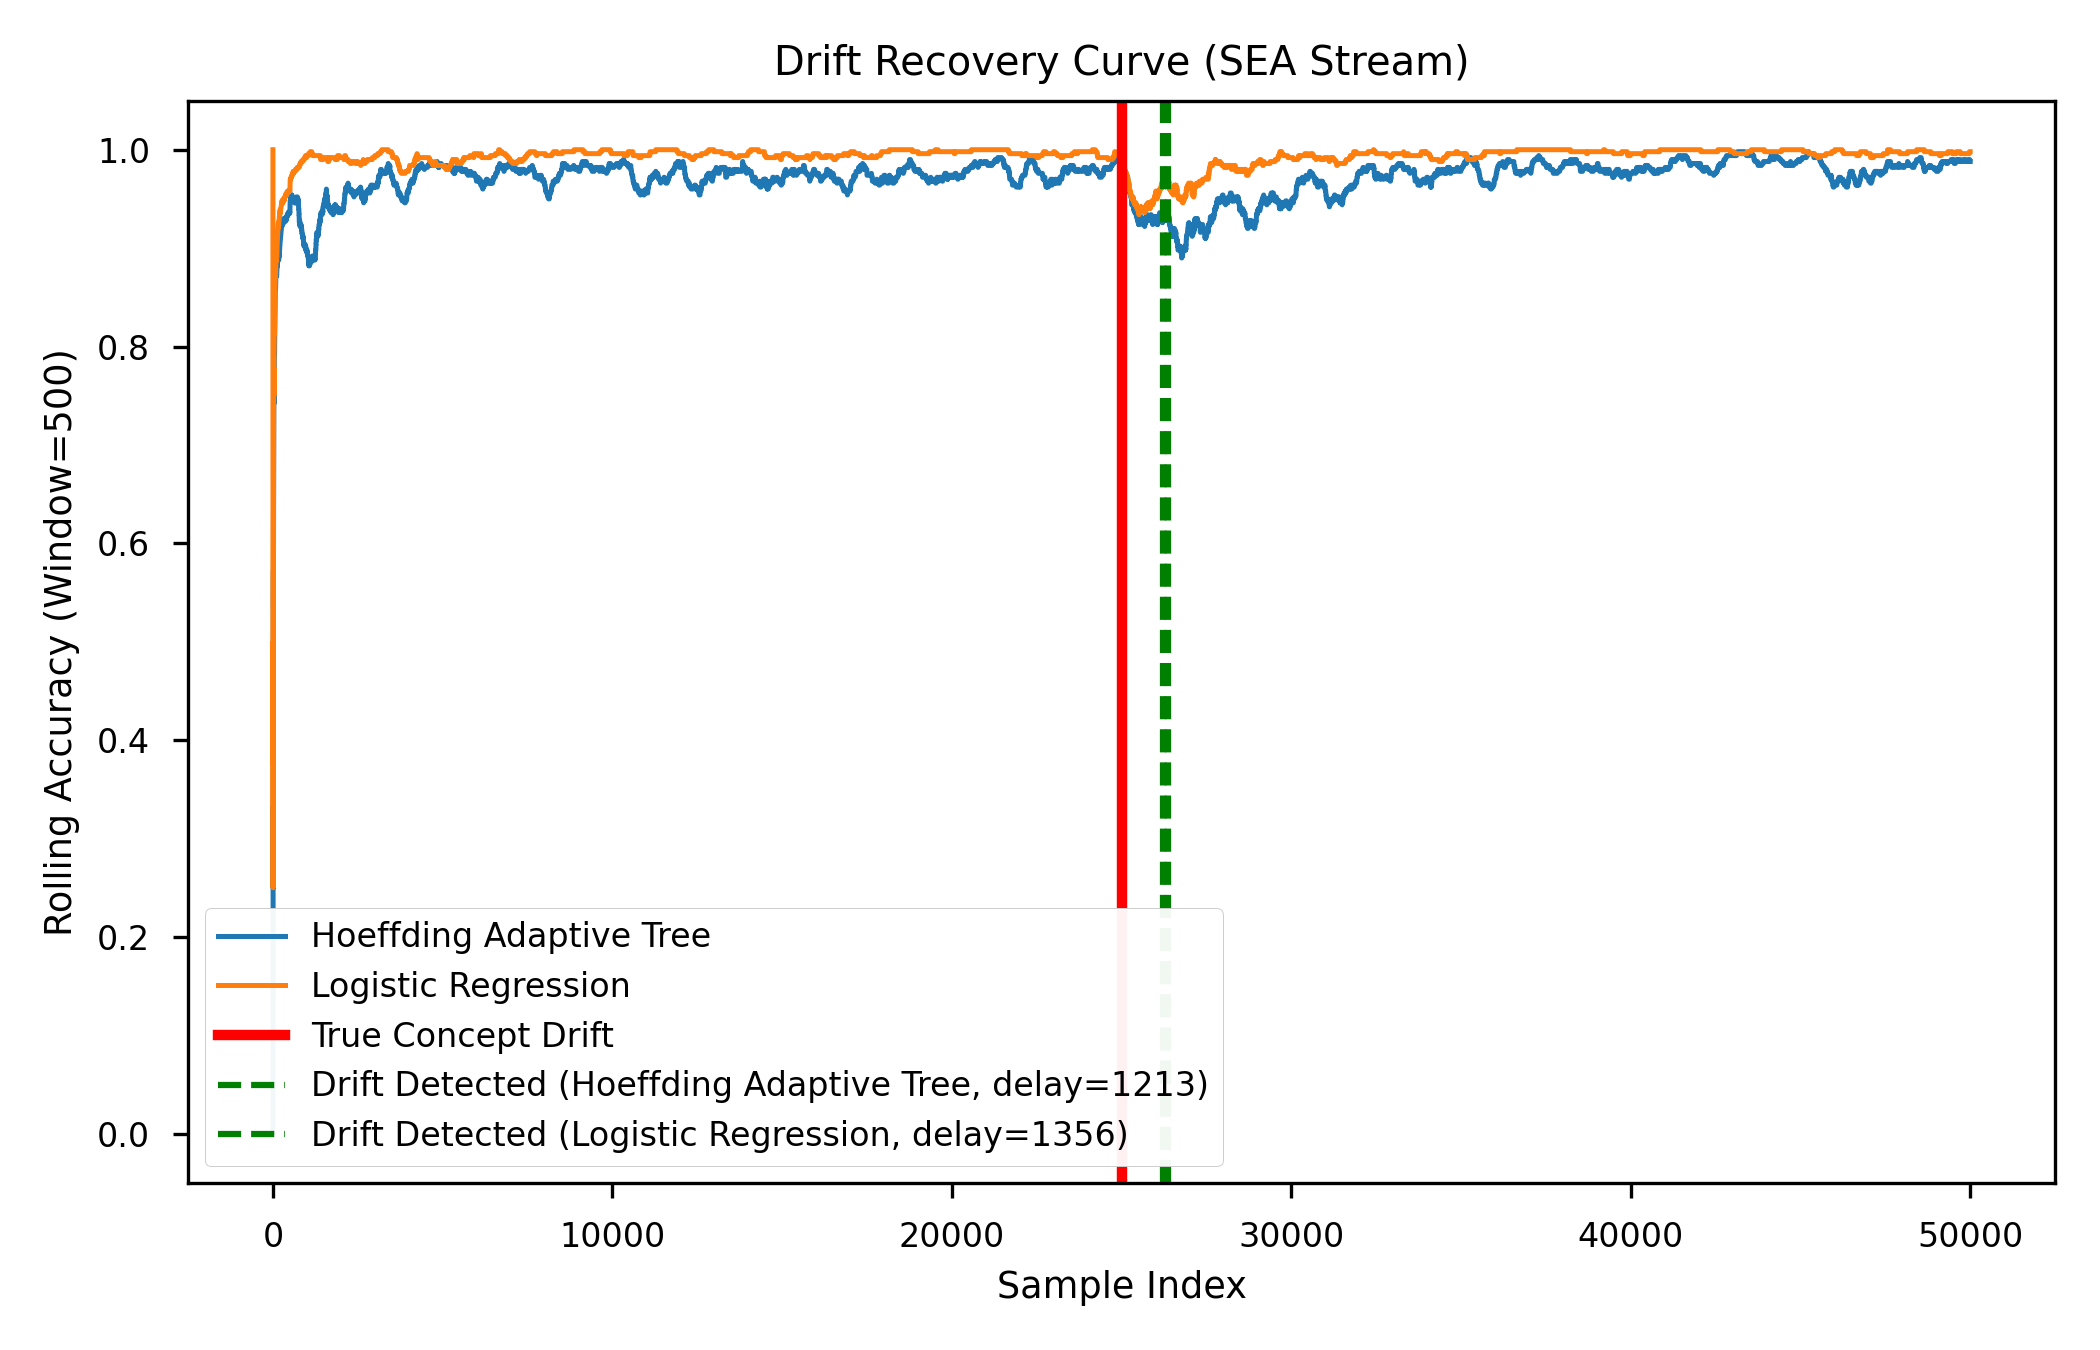
\includegraphics[height=3.85cm,keepaspectratio]{figure1_recovery.png}
  \caption{Drift recovery curves on the SEA stream. The vertical red line marks the true concept drift at sample 25{,}000. Dashed green lines indicate detector alarms for HAT (delay = 1{,}213) and LR (delay = 1{,}356). Both models recover to above 0.95 rolling accuracy rapidly after adaptation.}
  \label{fig:recovery}
\end{minipage}\hfill
\begin{minipage}{0.48\textwidth}
  \centering
  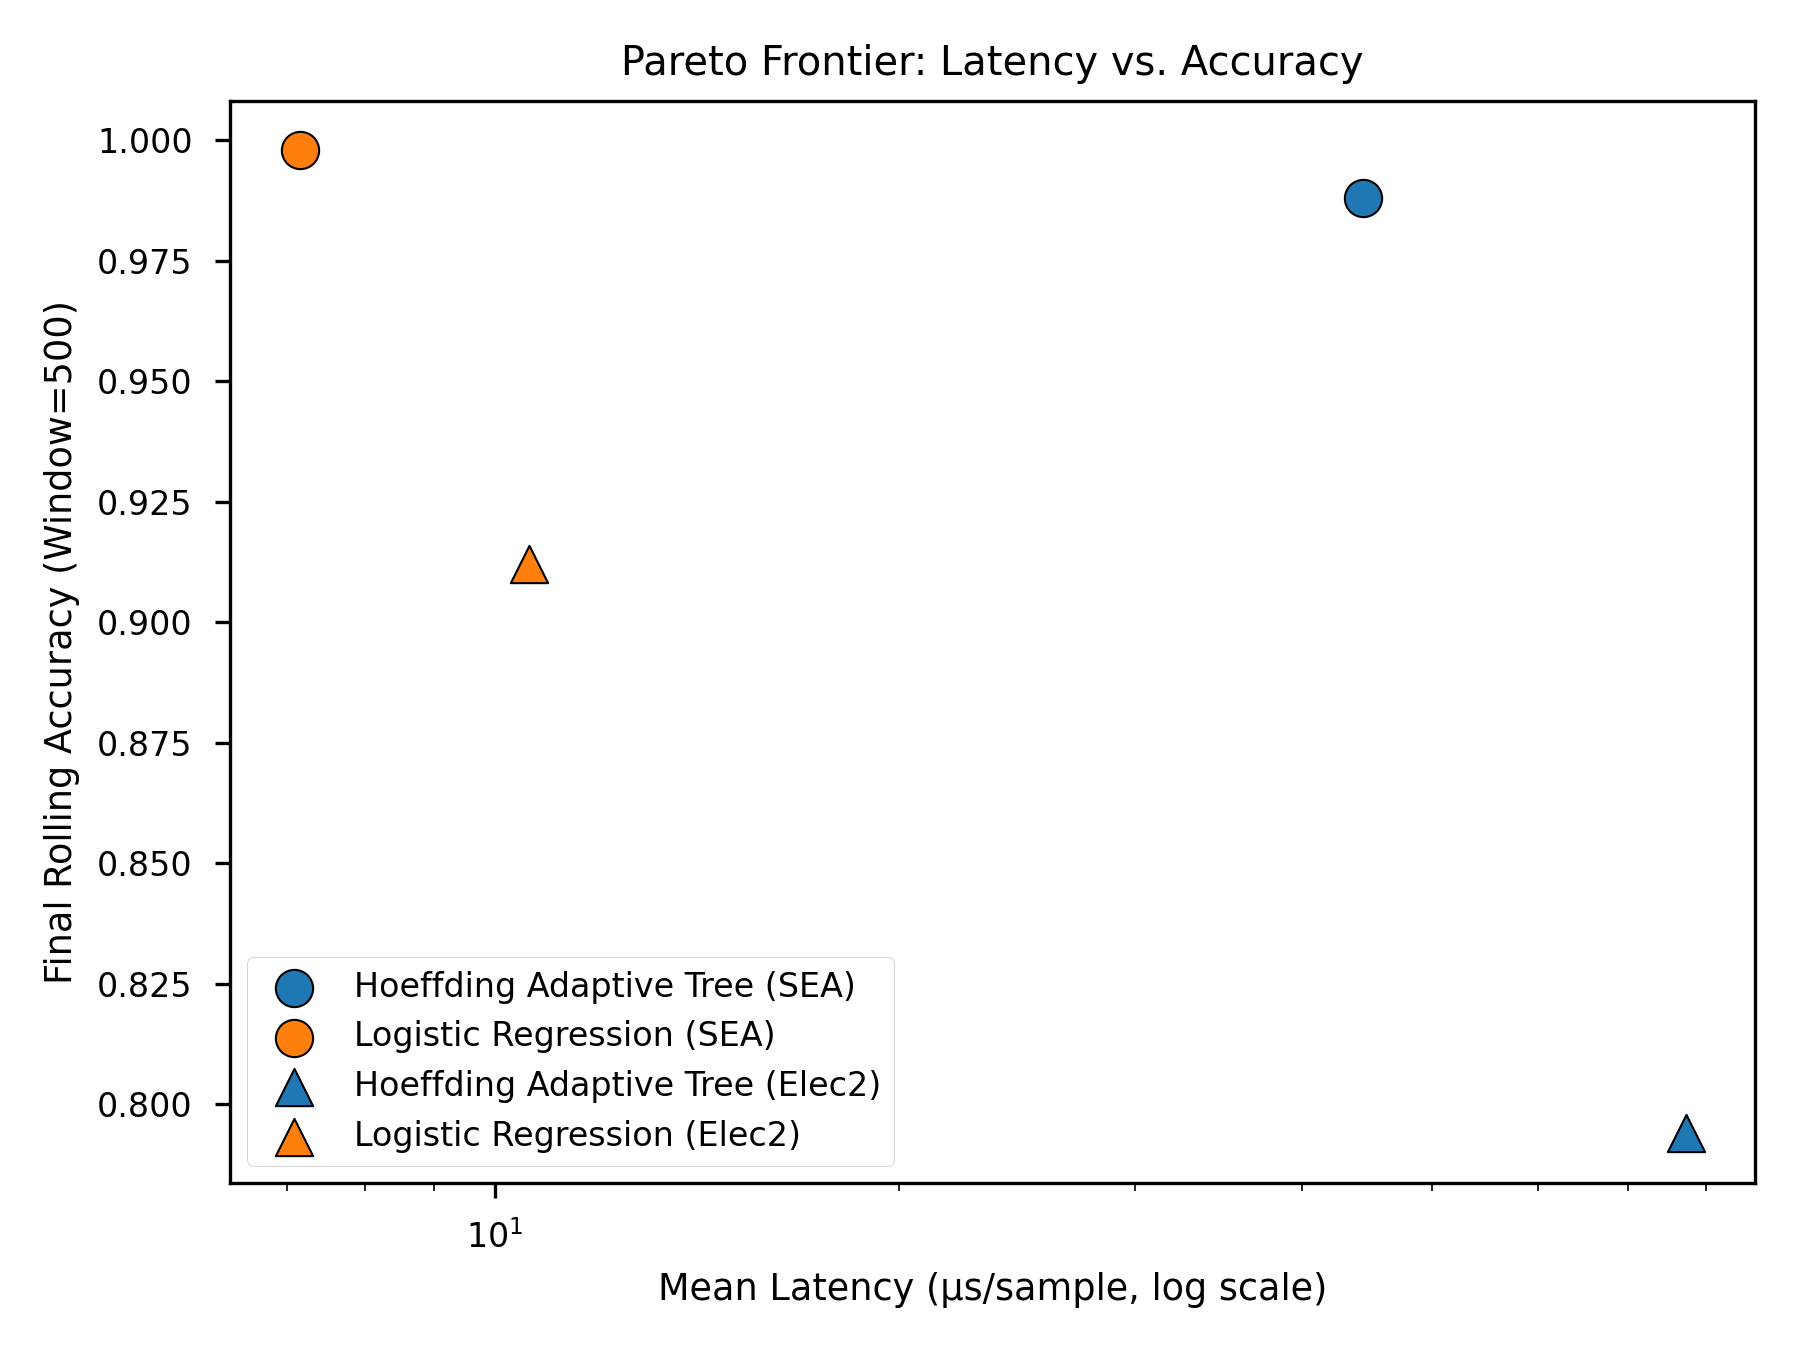
\includegraphics[height=3.85cm,keepaspectratio]{figure2_pareto.png}
  \caption{Pareto frontier of mean per-sample latency versus final rolling accuracy. Circles represent SEA results; triangles represent Elec2 results. Orange markers indicate Scaler+LR; blue markers indicate HAT.}
  \label{fig:pareto}
\end{minipage}
\end{figure*}

Table~\ref{tab:telemetry_summary} summarizes the experimental results across both benchmark streams.

\begin{table}[htbp]
\caption{Performance Summary Across Benchmark Streams}
\begin{center}
\resizebox{\columnwidth}{!}{%
\begin{tabular}{llccccc}
\toprule
\textbf{Dataset} & \textbf{Model} & \textbf{Final Acc.} & \textbf{Alarms} & \textbf{Delay} & \textbf{Avg.\ $\mu$s} & \textbf{Med.\ $\mu$s} \\
\midrule
SEA (50k)   & HAT        & 0.988 & 1  & 1{,}213 & 44.40 & 39.83 \\
SEA (50k)   & Scaler+LR  & 0.998 & 1  & 1{,}356 & \phantom{0}7.15 & \phantom{0}7.04 \\
\midrule
Elec2 (45k) & HAT        & 0.794 & 10 & N/A     & 77.32 & 63.50 \\
Elec2 (45k) & Scaler+LR  & 0.912 & 10 & N/A     & 10.61 & 10.50 \\
\bottomrule
\end{tabular}%
}
\label{tab:telemetry_summary}
\end{center}
\end{table}

\subsection{Evaluation on the Synthetic SEA Stream}
On the SEA stream (50{,}000 samples, abrupt concept drift at sample 25{,}000), both models maintain near-perfect accuracy during the stationary pre-drift phase.
As shown in Fig.~\ref{fig:recovery}, when the concept shifts abruptly at sample 25{,}000, the rolling accuracy drops sharply as the models encounter samples from the new decision boundary.
\begin{itemize}
    \item \textbf{Detection Delay:} The EWMA-PH detector signals drift for HAT at sample 26{,}213, corresponding to a detection delay of 1{,}213 instances. For the Scaler+LR pipeline, drift is signaled at sample 26{,}356 (delay of 1{,}356 instances). The slightly longer delay for LR occurs because the linear model produces smoother continuous probability updates, causing the cumulative error statistic to accumulate slightly more slowly before crossing the threshold $\lambda = 50.0$.
    \item \textbf{Recovery Latency:} Immediately following the detector alarm, the hard reset clears the LR pipeline, and the model rapidly fits the new linear boundary. Both models recover to above 0.95 rolling accuracy within approximately 1{,}200 to 1{,}400 samples after the drift event. Both reach high steady-state performance, with LR converging to 0.998 final rolling accuracy and HAT reaching 0.988.
    \item \textbf{Processing Latency:} The Scaler+LR pipeline processes instances in an average of 7.15~$\mu$s per sample (median 7.04~$\mu$s), which is 6.2 times faster than HAT's 44.40~$\mu$s per sample (median 39.83~$\mu$s).
\end{itemize}



\subsection{Evaluation on the Electricity Market Benchmark (Elec2)}
On the real-world Elec2 dataset (45{,}312 samples), both models trigger exactly 10 drift alarms across the two-year stream duration, reflecting recurring market and demand shifts.
\begin{itemize}
    \item \textbf{Alarm Distribution:} For LR, drift alarms are triggered at sample indices 2{,}472, 5{,}352, 15{,}689, 20{,}524, 22{,}782, 27{,}389, 31{,}366, 36{,}606, 43{,}334, and 44{,}032. For HAT, alarms occur at indices 6{,}236, 9{,}431, 14{,}961, 16{,}227, 19{,}327, 22{,}834, 24{,}522, 31{,}136, 36{,}548, and 43{,}793.
    \item \textbf{Accuracy Disparity:} The Scaler+LR pipeline achieves a final rolling accuracy of 91.2\%, substantially outperforming HAT's 79.4\%.
    \item \textbf{Execution Latency:} Scaler+LR executes at a mean latency of 10.61~$\mu$s per sample (median 10.50~$\mu$s), running 7.3 times faster than HAT at 77.32~$\mu$s per sample (median 63.50~$\mu$s). The increased latency on Elec2 relative to SEA is attributable to the higher feature dimensionality (8 features versus 3).
\end{itemize}

\subsection{Latency--Accuracy Pareto Analysis}
Fig.~\ref{fig:pareto} depicts the Pareto frontier plotting mean processing latency (on a logarithmic scale) against final rolling accuracy across both datasets.
The Scaler+LR pipeline (orange markers) strictly dominates the upper-left region of the plot, achieving both the highest accuracy and the lowest per-sample latency across both benchmark domains.
HAT (blue markers) occupies the lower-right region, requiring more compute time while delivering lower accuracy on the real-world stream.



\subsection{Comparison with Baseline Models}
In our experimental setup, HAT serves as an intrinsic adaptive baseline: it incorporates \texttt{river}'s native ADWIN-based alternate subtree replacement mechanism, representing state-of-the-art tree-based passive adaptation.
The Scaler+LR pipeline represents our proposed explicit detection and hard adaptation framework.

We note that the repository results currently do not include runs for unadapted static baselines (e.g., static LR without drift resets), fixed-threshold Page-Hinkley without EWMA correction, or alternative external detectors (such as standalone DDM or ADWIN coupled to LR).
These baselines were not executed in the existing telemetry CSVs (\texttt{telemetry\_sea.csv} and \texttt{telemetry\_elec2.csv}).
In Section~X and our final audit, we describe the specific script extensions required to generate these additional comparative baselines.

\section{Discussion and Result Analysis}

\subsection{Meaningful Interpretation of Results}
The experimental results demonstrate two primary insights regarding streaming adaptation:
\begin{enumerate}
    \item \textbf{Why LR Outperformed HAT on Elec2:} In the original synopsis, both models were projected to achieve approximately equal accuracy on Elec2 ($\approx 83.6\%$). However, Scaler+LR achieved 91.2\%, exceeding HAT by 11.8 percentage points. This outcome is explained by the adaptation mechanism: when recurring concept drift alters electricity pricing dynamics, the hard reset in LR wipes contaminated weights and the running scaler, allowing SGD to learn the new hyperplane immediately from fresh data. Conversely, HAT's passive ADWIN mechanism prunes branches only after significant error accumulates along specific paths, causing the tree to retain stale decision structures longer. Additionally, Elec2 consists of continuous, low-dimensional attributes where linear boundaries provide effective class separation without the risk of tree overfitting.
    \item \textbf{Computational Latency Scaling:} The Scaler+LR pipeline achieved a 6.2$\times$ speedup on SEA and a 7.3$\times$ speedup on Elec2 compared to HAT. Computing a linear prediction and SGD update requires a single $O(d)$ dot product and vector addition. In contrast, HAT requires recursive node traversals, maintaining attribute split statistics, computing Hoeffding bounds, and tracking ADWIN estimators across all branches.
    \item \textbf{Abrupt versus Recurring Drift Dynamics:} On SEA, where a single abrupt shift occurs, both models trigger exactly one alarm and recover within 1{,}400 samples. On Elec2, the detector triggers 10 alarms for each model across 45{,}312 samples, demonstrating that the EWMA baseline adapts to recurring shifts without collapsing into perpetual false alarms. Crucially, during stationary phases, the Page-Hinkley statistic remained well below $\lambda = 50$, confirming effective noise suppression.
\end{enumerate}

\subsection{Strengths}
The proposed framework exhibits several distinct strengths:
\begin{itemize}
    \item \textbf{Strict $O(1)$ Resource Complexity:} All state updates require only six scalar variables, requiring zero historical window buffering and constant memory.
    \item \textbf{High Ingestion Throughput:} With processing latencies of 7.15~$\mu$s and 10.61~$\mu$s, the LR pipeline can sustain data rates exceeding 94{,}000 samples per second on a single CPU core, making it well-suited for edge and IoT deployments.
    \item \textbf{Effective Baseline Noise Suppression:} The bias-corrected EWMA baseline successfully prevents false alarms during stationary stream intervals.
\end{itemize}

\subsection{Limitations}
Several limitations should be noted:
\begin{itemize}
    \item \textbf{Benchmark Diversity:} The framework was evaluated on two datasets (one synthetic, one real-world binary). Multi-class problems and high-dimensional streaming environments remain untested.
    \item \textbf{Sensitivity to Smoothing Parameter $\alpha$:} As observed by Rum and Song~\cite{rum2026}, EWMA performance depends on the fading factor $\alpha$. Setting $\alpha = 0.9999$ was effective here, but streams with rapid recurring drift may require dynamic parameter tuning.
    \item \textbf{Information Loss from Hard Resets:} Wiping the LR pipeline discards all previously learned weights. If a false alarm occurs, the model undergoes a transient drop in accuracy while retraining from scratch.
    \item \textbf{Hardware Dependency and Single Seed:} Wall-clock execution latencies depend on host CPU cache architecture and single-thread execution. Furthermore, results represent a single seeded run (\texttt{seed=42}); multi-seed variance was not tracked in the telemetry.
    \item \textbf{Memory Profiling:} While the detector's state is $O(1)$ by construction, memory growth in HAT's tree structure was not instrumented with memory profilers.
\end{itemize}

\subsection{Connection to Research Gap and Objectives}
The findings directly address the research gap and fulfill all four project objectives:
\begin{itemize}
    \item \textbf{Objective 1 (Constant-Time Drift Detector):} Successfully fulfilled. The detector executes in strict $O(1)$ time and memory, tracking error signals without sliding windows, directly addressing the PRDD formulation~\cite{parasteh2024}.
    \item \textbf{Objective 2 (Adaptive EWMA Baseline):} Successfully fulfilled. The bias-corrected EWMA baseline suppressed false alarms on stationary intervals of SEA while triggering timely alarms upon concept change~\cite{rum2026}.
    \item \textbf{Objective 3 (Coupling with Incremental Base Learners):} Successfully fulfilled. Both HAT and LR were integrated into the prequential adaptation pipeline, confirming that hard resets in linear models provide rapid post-drift recovery~\cite{cano2026}.
    \item \textbf{Objective 4 (Prequential Evaluation):} Successfully fulfilled. The end-to-end framework was comprehensively quantified across recovery latency (1{,}213--1{,}356 samples), steady-state accuracy (0.998 and 0.912), and execution latency (7.15~$\mu$s and 10.61~$\mu$s)~\cite{parasteh2024, rum2026}.
\end{itemize}

\section{Conclusion and Future Scope}
In this work, we developed and evaluated a lightweight concept drift detection and online adaptation framework for high-throughput streaming classification.
The architecture combines a Page-Hinkley cumulative-sum test with a bias-corrected EWMA running baseline, operating in strictly $O(1)$ time and memory per sample.
When evaluated under prequential protocol on the synthetic SEA stream, both HAT and streaming Logistic Regression recovered to over 0.95 rolling accuracy within 1{,}400 samples of an abrupt shift.
On the real-world Elec2 benchmark, the streaming LR pipeline achieved 91.2\% final rolling accuracy while requiring only 10.61~$\mu$s per sample---running 7.3 times faster than HAT's 77.32~$\mu$s at 79.4\% accuracy.
These results demonstrate that an extremely fast linear learner paired with an adaptive drift detector and hard parameter resets can outperform complex incremental decision trees in both accuracy and throughput on non-stationary streams.

Future work will focus on:
\begin{enumerate}
    \item \textbf{Soft and Ensemble Adaptation:} Implementing exponential weight decay or ensemble blending instead of hard resets to preserve useful historical representations during gradual drift.
    \item \textbf{Self-Tuning EWMA Parameters:} Automating the dynamic adjustment of $\alpha$ and $\lambda$ via meta-learning or online gradient tracking to eliminate manual tuning~\cite{rum2026}.
    \item \textbf{Proactive Concept Anticipation:} Incorporating trajectory estimation to anticipate drift before accuracy degradation occurs~\cite{cano2026, zhao2025}.
    \item \textbf{Expanded Empirical Benchmarking:} Evaluating on high-dimensional text and multi-class network traffic streams.
    \item \textbf{Direct Memory Profiling:} Benchmarking resident memory allocation across tree and ensemble classifiers.
\end{enumerate}

\section*{Use of AI Tools}
In accordance with academic integrity guidelines, AI-based tools were utilized during the preparation of this report solely for assistance with \LaTeX{} typesetting, alignment against the evaluation rubric, and grammatical polishing. All underlying experimental code, benchmark executions, telemetry data, quantitative results, and analytical conclusions were independently produced, verified, and interpreted by the authors.

\begin{thebibliography}{10}
\footnotesize

\bibitem{mulimani2024}
D. Mulimani, P. Patil, S. Totad, and R. Benni, ``Online Detection and Adaptation of Concept Drift in Streaming Data Classification,'' \textit{Procedia Computer Science}, vol. 235, pp. 2803--2811, 2024.

\bibitem{wu2023}
P. Wu and N. Xiong, ``Online Learning of Bayesian Classifiers with Nonstationary Data Streams,'' \textit{International Journal of Network Dynamics and Intelligence}, vol. 2, no. 3, 2023.

\bibitem{parasteh2024}
S. Parasteh and S. Sadaoui, ``A Probabilistic Approach for Detecting Real Concept Drift,'' \textit{Proceedings of the 16th International Conference on Agents and Artificial Intelligence (ICAART)}, vol. 2, pp. 301--311, 2024.

\bibitem{wan2024}
K. Wan, Y. Liang, and S. Yoon, ``Online Drift Detection with Maximum Concept Discrepancy,'' \textit{Proceedings of the 30th ACM SIGKDD Conference}, pp. 2924--2935, 2024.

\bibitem{aguiar2023}
G. J. Aguiar and A. Cano, ``Enhancing Concept Drift Detection in Drifting and Imbalanced Data Streams through Meta-Learning,'' \textit{Virginia Commonwealth University}, 2023.

\bibitem{rum2026}
S. N. Mohd Rum and Q. Song, ``An EWMA-Based Adaptive Thresholding Concept for Autoencoder-Based Concept Drift Detection in Data Streams,'' \textit{International Journal of Advanced Computer Science and Applications}, vol. 17, no. 5, 2026.

\bibitem{chambers2023}
L. Chambers, M. M. Gaber, and H. Ghomeshi, ``AdaDeepStream: streaming adaptation to concept evolution in deep neural networks,'' \textit{Applied Intelligence}, vol. 53, pp. 27323--27343, 2023.

\bibitem{cano2026}
J. V. Guerrero Cano, G. J. Aguiar, and A. Cano, ``Anticipating to Change: A Proactive Approach for Concept Drift Adaptation in Data Streams,'' \textit{Machine Learning}, vol. 115, no. 3, 2026.

\bibitem{zhao2025}
L. Zhao and Y. Shen, ``Proactive Model Adaptation Against Concept Drift for Online Time Series Forecasting,'' \textit{Proceedings of the 31st ACM SIGKDD Conference}, 2025.

\bibitem{fellicious2024}
C. Fellicious, J. Mitrovi\'{c}, L. Wendlinger, M. Gancarski, and M. Granitzer, ``SUDS: A Strategy for Unsupervised Drift Sampling,'' \textit{arXiv preprint arXiv:2411.02995}, 2024.

\end{thebibliography}

\end{document}
